\documentclass[11pt,a4paper]{article}

\usepackage[T1]{fontenc}
\usepackage[utf8]{inputenc}
\usepackage{lmodern}
\usepackage[margin=2.2cm]{geometry}
\usepackage{microtype}
\usepackage{amsmath}
\usepackage{graphicx}
\usepackage{booktabs}
\usepackage{float}
\usepackage[font=small,labelfont=bf]{caption}
\usepackage{xcolor}
\usepackage[colorlinks=true,linkcolor=blue!50!black,urlcolor=blue!50!black,citecolor=blue!50!black]{hyperref}

\graphicspath{{../figures/}}
\setlength{\parskip}{0.35em}
\setlength{\parindent}{0pt}
\captionsetup{skip=4pt}
\setlength{\textfloatsep}{10pt plus 2pt minus 2pt}
\setlength{\floatsep}{8pt plus 2pt minus 2pt}

\title{\textbf{Road accidents in France, 2005--2025}\\[0.3em]
\large Who gets seriously hurt, where and why: data engineering, statistics and machine learning}
\author{Mouataz Bounit}
\date{}

\begin{document}
\maketitle
\vspace{-2.5em}

\begin{abstract}
\noindent
This report analyses the 1.34 million injury road accidents recorded by the French police between 2005
and 2025 (3.0 million people involved). The 84 official files are harmonised into one schema, checked for
quality and joined correctly, which reveals that the naive join used in a first version of this work
inflated every count by 90\%. Exploration and per-capita maps show that the mode of transport, the
other party, rural roads and night-time drive the severity of injuries. A logistic regression with
errors clustered by accident quantifies these effects all else equal, and machine learning models trained
on 2019--2022 and tested on 2024--2025 reach a ROC-AUC of 0.846 (XGBoost), against 0.825 for the
penalised logistic regression. The whole pipeline is reproducible and comes with an interactive dashboard.
\end{abstract}

%==========================================================================================
\section{Introduction}

France recorded 3,442 road deaths in 2025. The number fell steadily until 2013 and has barely moved
since, while the casualties remain very unevenly shared between road users. This project asks a single
question:

\begin{center}
\emph{Given that an injury accident has happened, which factors make it more likely that a person\\ is
killed or hospitalised?}
\end{center}

The question is about \emph{severity}, not about the risk of having an accident: the data only contains
accidents with at least one injured person, and no exposure measure (kilometres travelled by mode) is
available. Every part of the work points to this question: the data engineering builds a reliable
person-level table, the exploration and the maps describe the contrasts, the logistic regression
measures each factor all else equal, and the machine learning models test how well severity can be
predicted on years they have never seen.

%==========================================================================================
\section{Data}

ONISR, the French road safety observatory, publishes every year the \emph{Bulletins d'Analyse des
Accidents Corporels} (BAAC) filled in by the police for each injury accident \cite{onisr}. Each year
comes as four tables linked by the accident number (Table~\ref{tab:tables}). Population estimates by
department come from INSEE and department boundaries from IGN.

\begin{table}[H]
\centering\footnotesize
\caption{The four BAAC tables.}
\label{tab:tables}
\begin{tabular}{@{}lll@{}}
\toprule
Table & One row per & Main variables \\
\midrule
Characteristics & accident & date, time, lighting, weather, built-up area, intersection, collision, department \\
Places & accident & road category, speed limit, surface, layout \\
Vehicles & vehicle & category, obstacle hit, impact point, manoeuvre \\
Users & person & role, sex, year of birth, severity, safety equipment, trip purpose \\
\bottomrule
\end{tabular}
\end{table}

Severity follows the official definitions: \emph{killed} means died within 30 days,
\emph{hospitalised} means admitted for more than 24 hours, \emph{slightly injured} means treated without
such an admission. The target of the models is a person being killed or hospitalised (\emph{severe}).

Two breaks in the data shape the analysis. First, ONISR warns that ``hospitalised'' is recorded
differently from 2018 and cannot be compared with earlier years; the number of hospitalised people
indeed falls by 24\% between 2017 and 2018 while deaths barely move. Second, vehicle categories and
safety equipment are recoded in 2019 (e-scooters and e-bikes appear). Counts are therefore shown over
2005--2025, but severity rates and all models use \textbf{2019--2025} only.

%==========================================================================================
\section{Data engineering}

\paragraph{Harmonisation.} The 84 raw files (470\,MB) change format several times: the separator goes
from comma to semicolon, the encoding from latin1 to UTF-8, the accident key is renamed in 2022, the time
of day is written \texttt{1930} and later \texttt{19:30}, departments use three digits before 2019
(\texttt{590} for Nord, \texttt{201} for Corse-du-Sud) and coordinates switch from degrees $\times 10^5$,
with \texttt{0000000} for missing values, to decimal degrees. A script detects the format of each file and
produces one schema with consistent names and types.

\paragraph{Quality checks.} Table~\ref{tab:quality} lists the main checks and how each one is handled.
Overseas collectivities, which only appear from 2019, are excluded so that the series stay comparable;
the scope is mainland France and the five overseas departments.

\begin{table}[H]
\centering\small
\caption{Main quality checks (rows over 2005--2025).}
\label{tab:quality}
\begin{tabular}{@{}lrl@{}}
\toprule
Check & Rows & Action \\
\midrule
Accidents in overseas collectivities (recorded from 2019 only) & 3,464 & excluded \\
Several place rows for one accident (from 2023) & 47,599 & main road kept \\
Duplicated vehicle letters within an accident (from 2019) & 54 & join on unique vehicle id \\
Users whose vehicle is missing & 22 & kept, vehicle variables missing \\
Age below 0 or above 105 & 395 & set to missing \\
Unknown severity (mostly hit-and-run users, from 2021) & 418 & excluded from severity analyses \\
Coordinates outside mainland France & 11 & set to missing \\
\bottomrule
\end{tabular}
\end{table}

\paragraph{Joins.} Each person must be linked to \emph{their own} vehicle (a pedestrian to the vehicle
that hit them): with the unique vehicle identifier from 2019, with the vehicle letter before. Joining
users and vehicles on the accident number alone pairs every person with every vehicle of the accident and
produces 5,703,904 rows instead of 3,005,246 (+90\%). This was the main error of the first version of
the project. Six automatic tests now check that every person and every accident is kept exactly once and
that the number of deaths matches the accident totals.

\paragraph{Features.} Age and age group, period of the day, vehicle groups mapped across the two
vehicle nomenclatures, the person's \emph{mode} (their vehicle, or \emph{pedestrian}), the
\emph{heaviest other party} in the accident (from bicycle to heavy goods vehicle), the use of a belt or
helmet, speed-limit classes and the binary target.

%==========================================================================================
\section{Exploratory analysis}

Deaths fell from 5,543 in 2005 to 3,427 in 2013 ($-38\%$), then stayed between 3,100 and 3,700 apart from
the 2020 lockdowns (Figure~\ref{fig:trend}). Car occupant deaths halved since 2005 (3,173 to 1,615) while
cyclist deaths rose by 32\% (187 to 246).

\begin{figure}[H]
\centering
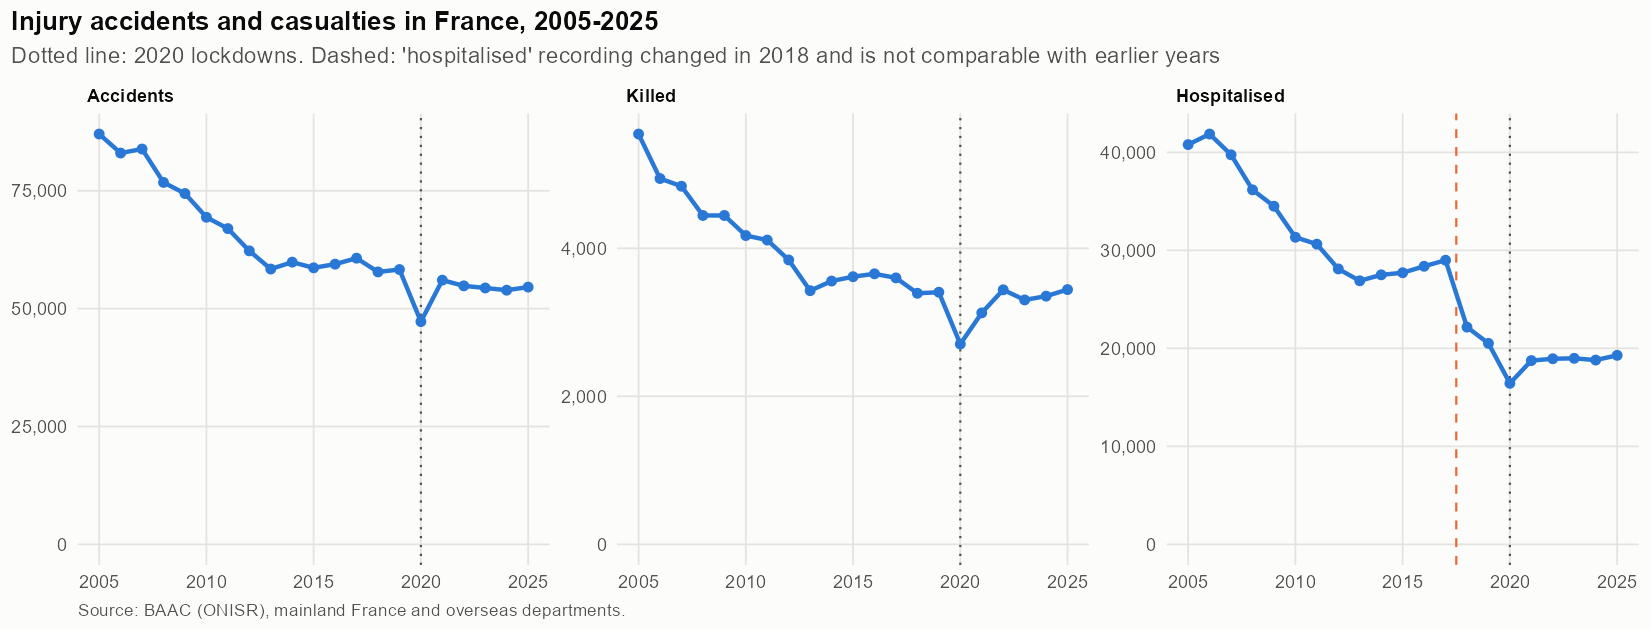
\includegraphics[width=\textwidth]{03_eda/01_yearly_trend.png}
\caption{Injury accidents and casualties per year. The dashed line marks the 2018 change in how
hospitalised people are recorded; the dotted line the 2020 lockdowns.}
\label{fig:trend}
\end{figure}

The mode of transport dominates every other contrast (Figure~\ref{fig:modes}): between 2019 and 2025,
37\% of motorcyclists, 33\% of pedestrians and 28\% of cyclists involved in an accident were killed or
hospitalised, against 12.5\% of car occupants. The other party matters as much: hit by a heavy goods
vehicle, 64\% of pedestrians and 55\% of cyclists are severely hurt, and a motorcyclist who crashes alone
is as badly hurt as one hit by a lorry (47\%) (Figure~\ref{fig:opponent}).

\begin{figure}[H]
\centering
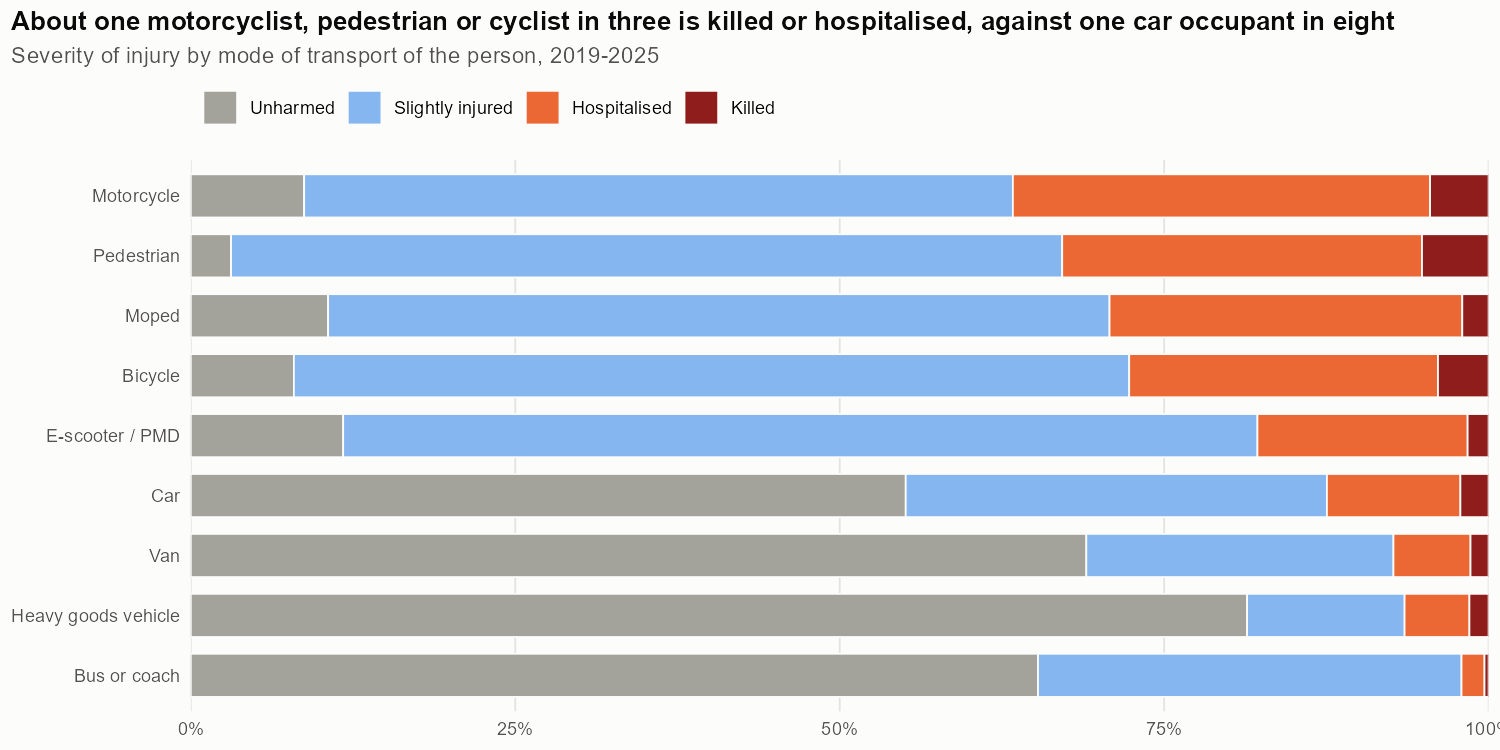
\includegraphics[width=0.86\textwidth]{03_eda/07_mode_severity.png}
\caption{Severity of injury by mode of transport, 2019--2025.}
\label{fig:modes}
\end{figure}

\begin{figure}[H]
\centering
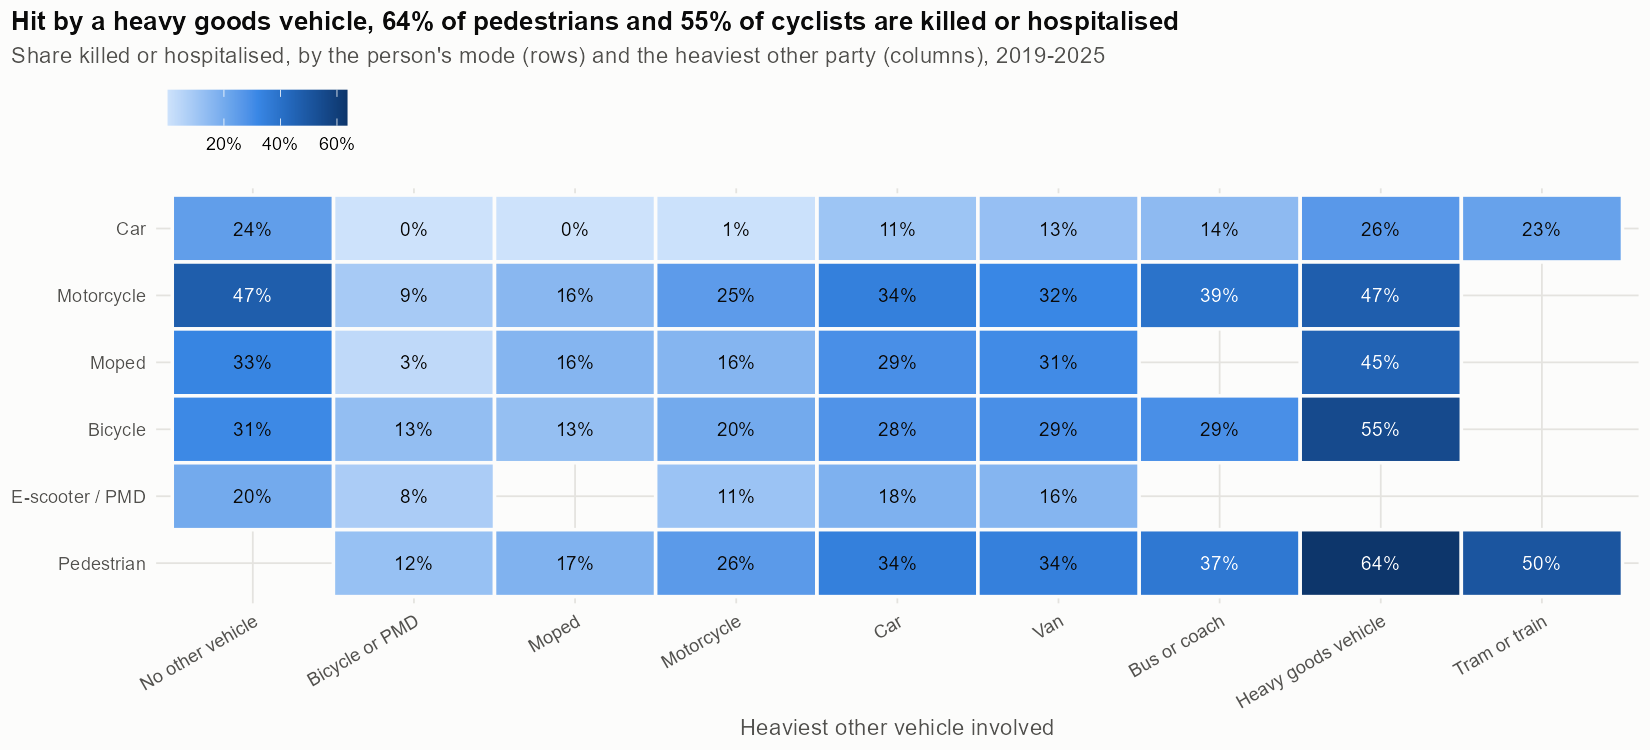
\includegraphics[width=0.86\textwidth]{03_eda/10_opponent.png}
\caption{Share killed or hospitalised by the person's mode (rows) and the heaviest other vehicle
involved (columns), 2019--2025.}
\label{fig:opponent}
\end{figure}

Time and place add strong gradients. Between 3 and 5~a.m., an accident kills 2 to 3 times as often as
at 5~p.m. On departmental roads outside built-up areas there are 14.5 deaths per 100 accidents, against
4.3 on the same roads in town. At night on unlit roads, the share of people killed is 2.7 times the
daylight level. Nearly four road deaths in five are men, and people over 75 are the most fragile once
involved. Light rain is associated with \emph{less} severe accidents, a reminder that these are raw
contrasts: drivers slow down and rainy accidents happen more often in towns.

%==========================================================================================
\section{Geography}

Raw counts by department mostly reflect population, so the maps show rates (Figure~\ref{fig:maps}).
Over 2021--2025, mainland France counts 79 injury accidents per 100,000 inhabitants and 48 deaths per
million per year. Paris has the most accidents per inhabitant but an accident there kills 0.8 people per
100, against 17.6 in Haute-Marne; deaths per million range from 14 in Hauts-de-Seine to 115 in
Haute-Marne. Dense departments have many accidents but few deaths per accident; rural departments of the
centre and north-east the opposite. Since 2010--2014, deaths per million have fallen in most departments
but risen in a few rural ones (Nièvre, Aube, Haute-Marne) and in Brittany.

\begin{figure}[H]
\centering
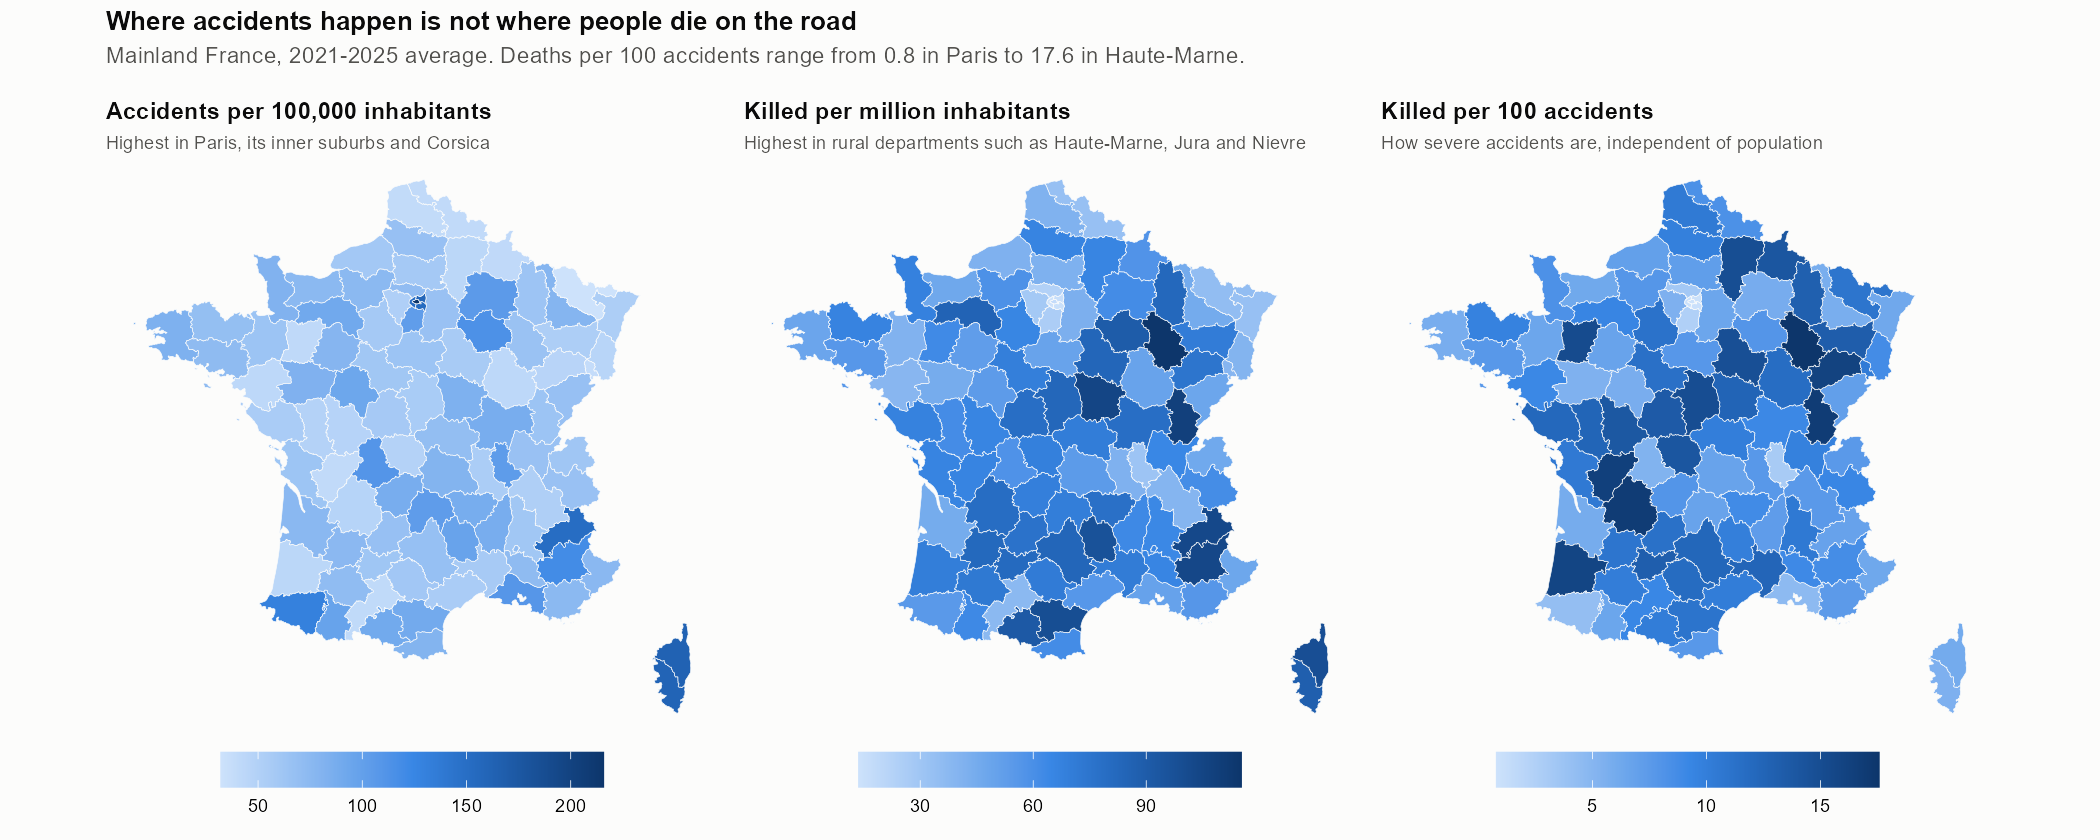
\includegraphics[width=\textwidth]{04_geography/01_department_maps.png}
\caption{Accidents per 100,000 inhabitants, deaths per million inhabitants and deaths per 100 accidents,
mainland France, 2021--2025 average.}
\label{fig:maps}
\end{figure}

%==========================================================================================
\section{Statistical model: logistic regression}

\paragraph{Specification.} For each person $i$ involved in an accident in year $t \in \{2019,\dots,2025\}$,
\begin{equation}
\operatorname{logit} P(\text{severe}_i = 1) = \alpha_t + \boldsymbol{x}_i^\top \boldsymbol{\beta},
\end{equation}
with year fixed effects $\alpha_t$ and covariates $\boldsymbol{x}_i$ known \emph{before} the impact: mode,
passenger, sex, age group, belt or helmet, heaviest other party, road category, built-up area, speed
limit, intersection, lighting, weather, surface, time of day, weekend and overseas. Collision type,
obstacle and impact point describe the crash itself and are deliberately left out, so that the model
describes who is at risk in which situation. People in the same accident share the road, the speed and
the impact, so standard errors are clustered by accident \cite{cameron}; they are 11\% wider than the
naive ones in median.

\paragraph{Results.} The model is estimated on 841,052 people in 377,178 accidents (18.1\% severe), with an
in-sample ROC-AUC of 0.829 and a McFadden pseudo-$R^2$ of 0.238. Table~\ref{tab:or} reports the main odds
ratios.

\begin{table}[H]
\centering\small
\caption{Odds ratios of being killed or hospitalised, all other factors held equal (95\% intervals
clustered by accident).}
\label{tab:or}
\begin{tabular}{@{}llr@{}}
\toprule
Factor & Reference & Odds ratio [95\% CI] \\
\midrule
Pedestrian & car occupant & 10.03 [9.77--10.30] \\
Motorcyclist & car occupant & 6.49 [6.35--6.63] \\
Cyclist & car occupant & 4.02 [3.89--4.15] \\
Belt or helmet not worn & worn & 4.30 [4.13--4.47] \\
Aged 75 or more & 35--44 & 3.29 [3.19--3.39] \\
Heaviest other party: heavy goods vehicle & car & 2.69 [2.59--2.79] \\
No other vehicle involved & car & 1.94 [1.91--1.98] \\
Outside a built-up area & built-up area & 2.51 [2.44--2.58] \\
Night (22h--6h) & 10h--16h & 1.56 [1.51--1.61] \\
Night without street lights & daylight & 1.23 [1.20--1.27] \\
Man & woman & 1.05 [1.03--1.06] \\
\bottomrule
\end{tabular}
\end{table}

Two raw contrasts shrink once the other factors are held equal. Unlit roads at night, which multiplied the
share of people killed by 2.7, keep an odds ratio of 1.23: most of their effect came from night-time and
rural roads. Men are 78\% of the dead but barely more likely than women to be seriously hurt in the same
kind of accident (1.05): the difference comes from exposure and behaviour, not from the outcome of a given
crash. Correlated variables must be read together: the 130\,km/h limit has a high odds ratio (4.88) but
only occurs on motorways, whose own odds ratio is 0.28.

\paragraph{Interactions.} Adding mode $\times$ built-up area and age $\times$ pedestrian improves the model
significantly (Wald tests, $p < 10^{-40}$). Average predicted probabilities, where every person is given
each level in turn, make them readable: leaving built-up areas raises the probability of a severe outcome
from 32\% to 50\% for pedestrians, from 20\% to 37\% for cyclists and from 6\% to 15\% for belted car
occupants; from age 35--44 to 75 and over it rises by 24 points for pedestrians and 12 points for belted
car occupants (Figure~\ref{fig:inter}).

\begin{figure}[tbp]
\centering
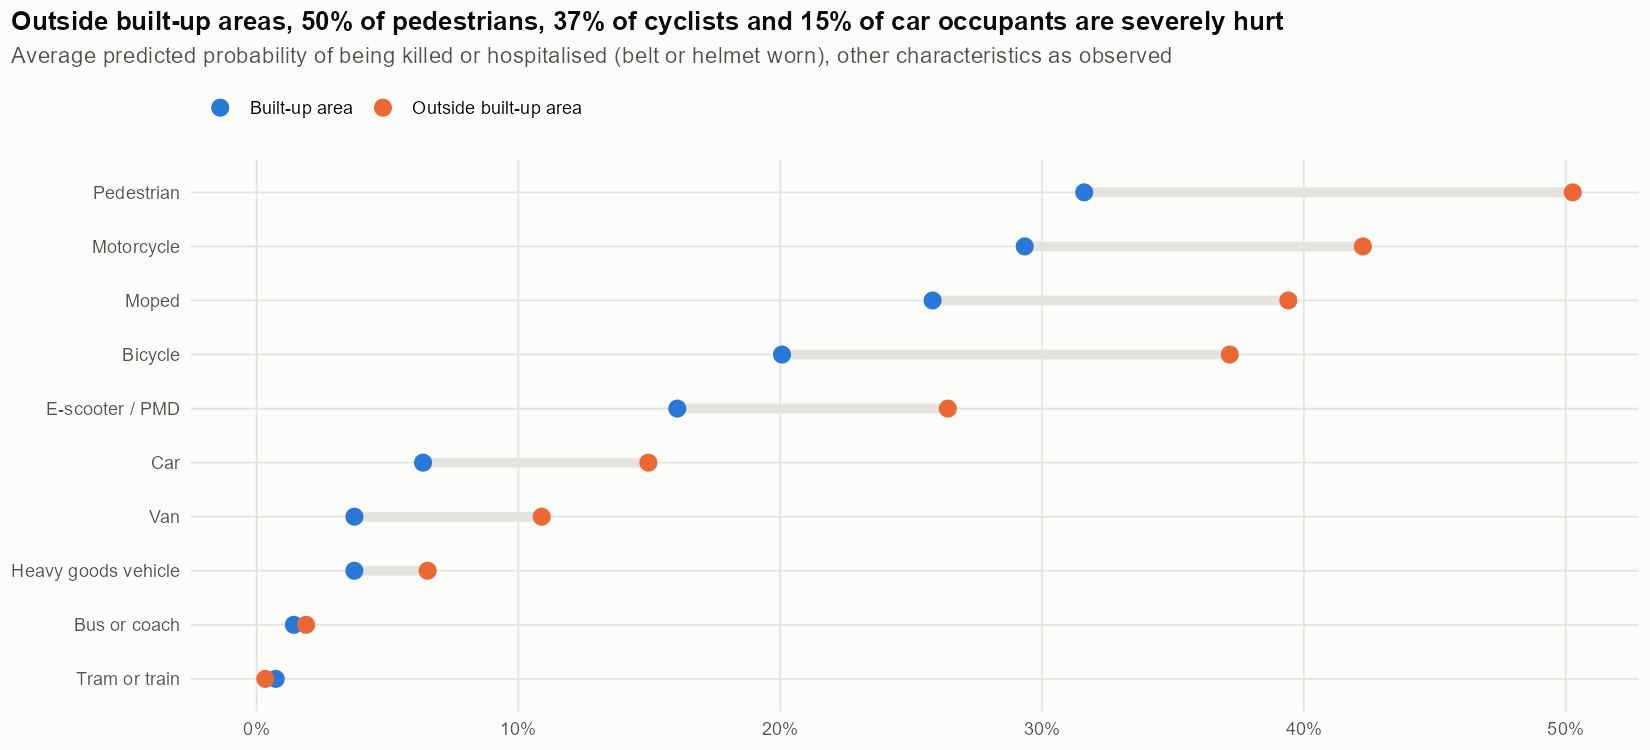
\includegraphics[width=0.495\textwidth]{05_model/02_mode_by_location.png}\hfill
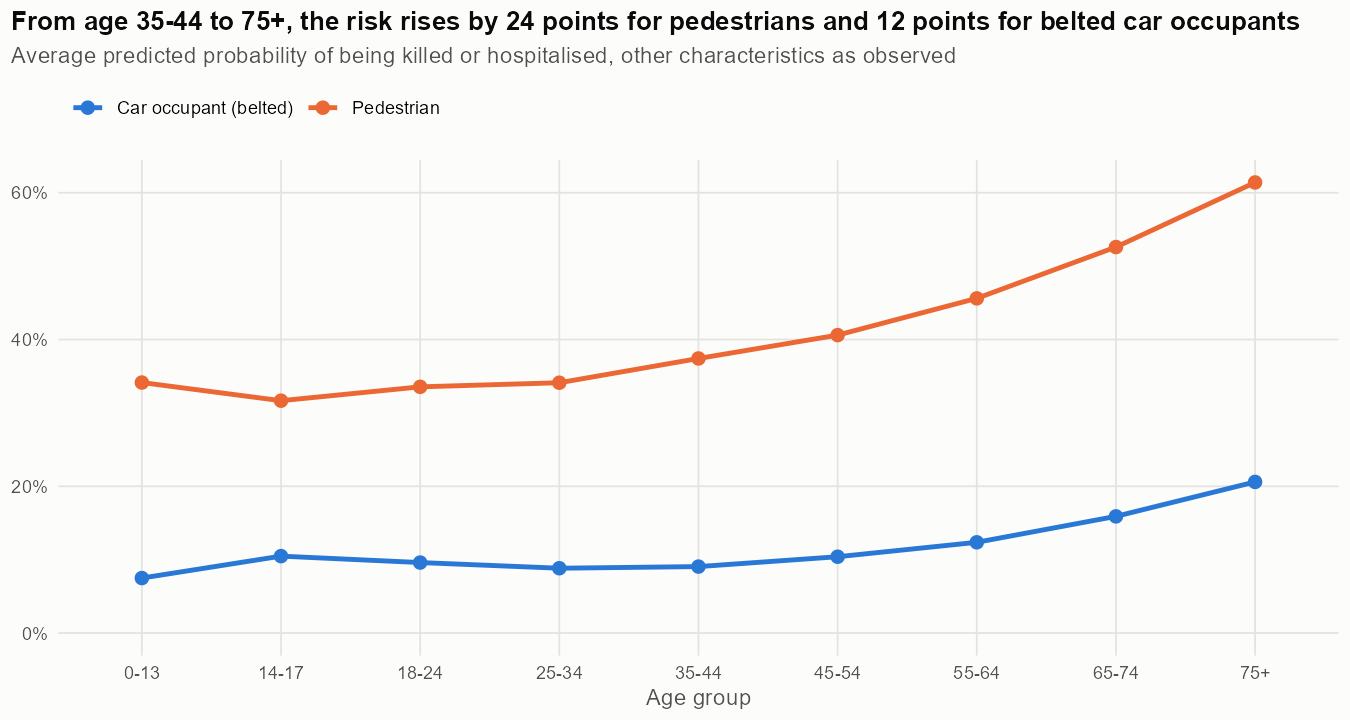
\includegraphics[width=0.495\textwidth]{05_model/03_age_pedestrian.png}
\caption{Average predicted probability of being killed or hospitalised from the model with interactions:
by mode inside and outside built-up areas (left), by age for pedestrians and belted car occupants (right).}
\label{fig:inter}
\end{figure}

%==========================================================================================
\section{Machine learning and evaluation}

\paragraph{Set-up.} The population and target are those of the logistic regression. The split is
chronological, so that models are judged on years they have never seen: training on 2019--2022 (478,236
people), validation on 2023 (120,808) for tuning, early stopping and decision thresholds, and test on
2024--2025 (242,008). Final models are refitted on 2019--2023 with the tuned settings. Five models are
compared: a prevalence baseline, a ``rate by mode'' rule, a penalised logistic regression (glmnet
\cite{glmnet}, $\alpha$ and $\lambda$ chosen on the 2023 log loss), a random forest (ranger
\cite{ranger}) and XGBoost \cite{xgboost} (depth 8, learning rate 0.05, 484 rounds by early stopping).
The two best are also refitted with the crash variables. Confidence intervals come from 200 bootstrap
samples of \emph{whole accidents}.

\begin{table}[H]
\centering\small
\caption{Performance on the test years 2024--2025 (18.3\% killed or hospitalised).}
\label{tab:ml}
\begin{tabular}{@{}lcccc@{}}
\toprule
Model & ROC-AUC [95\% CI] & PR-AUC & Log loss & Brier \\
\midrule
Baseline: prevalence & 0.500 & 0.183 & 0.476 & 0.150 \\
Baseline: rate by mode & 0.669 [0.666--0.673] & 0.308 & 0.444 & 0.140 \\
Penalised logistic regression & 0.825 [0.823--0.827] & 0.516 & 0.366 & 0.116 \\
Random forest & 0.843 [0.841--0.844] & 0.548 & 0.351 & 0.111 \\
\textbf{XGBoost} & \textbf{0.846 [0.844--0.848]} & \textbf{0.555} & \textbf{0.348} & \textbf{0.111} \\
\midrule
Penalised logistic + crash variables & 0.846 [0.844--0.848] & 0.546 & 0.350 & 0.111 \\
XGBoost + crash variables & 0.869 [0.867--0.871] & 0.600 & 0.326 & 0.104 \\
\bottomrule
\end{tabular}
\end{table}

\paragraph{Results.} XGBoost ranks people best (Table~\ref{tab:ml}, Figure~\ref{fig:roc}). Its gain over
the logistic regression is small but certain: $+0.020$ of ROC-AUC (paired bootstrap interval
$[0.020, 0.022]$) and $+0.040$ of PR-AUC. Adding the crash variables raises the ROC-AUC to 0.869, which
shows how much of the outcome is decided by the crash itself. All models are well calibrated, with a mean
gap between predicted and observed rates below one percentage point, and performance is stable between
2024 (0.847) and 2025 (0.844).

\begin{figure}[H]
\centering
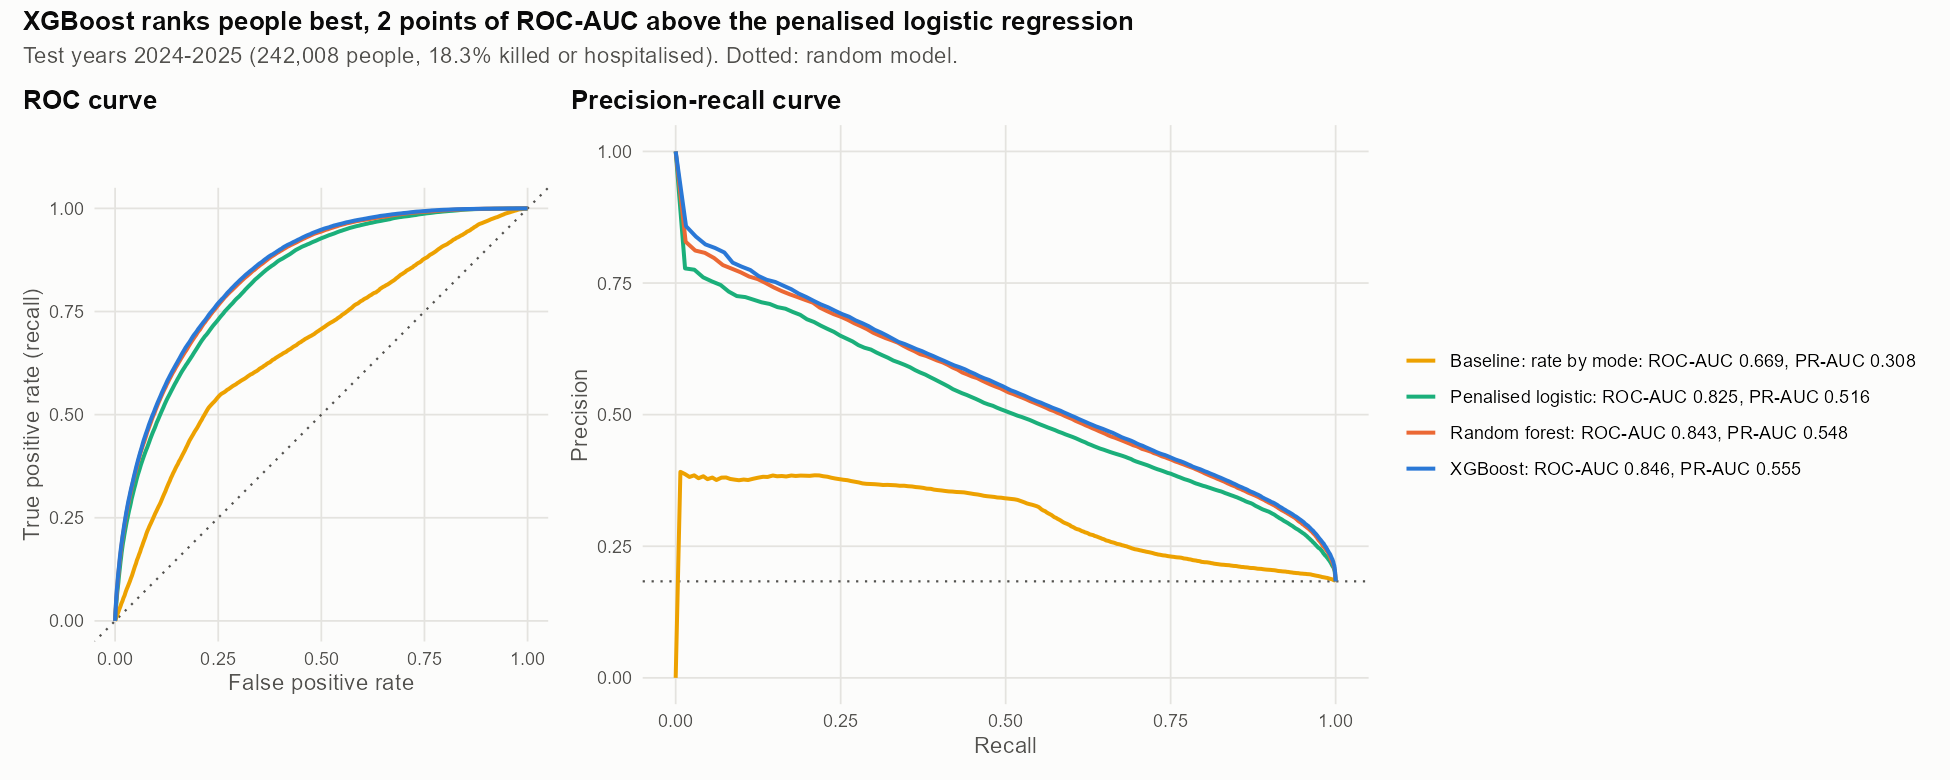
\includegraphics[width=\textwidth]{07_evaluation/01_roc_pr_curves.png}
\caption{ROC and precision-recall curves on 2024--2025. Dotted lines: random model.}
\label{fig:roc}
\end{figure}

\paragraph{Decisions and errors.} With a threshold chosen on 2023 to maximise F1, XGBoost flags 25\% of
people, with a precision of 47\% and a recall of 65\% (F1 = 0.55, against 0.52 for the logistic
regression). The global score hides a limit: \emph{within} a mode, severity is much harder to predict for
vulnerable road users (ROC-AUC 0.73 for pedestrians, 0.75 for motorcyclists, 0.68 for e-scooter riders)
than for car occupants (0.86). The model misses 43\% of severe car occupants and 67\% of severe e-scooter
riders, whose predicted risk is low on average.

\paragraph{Interpretability.} SHAP values \cite{shap} computed on the final XGBoost rank the mode of
transport first, then the heaviest other party, the road category and the built-up area
(Figure~\ref{fig:shap}). Not wearing a belt or helmet has one of the largest odds ratios but a modest
mean SHAP value: it is rare, so it matters a lot for few people. One technical point mattered: XGBoost
treats the unstored zeros of a sparse matrix as missing values, so SHAP values must be computed on the
same sparse representation as the training data, otherwise they are wrong.

\begin{figure}[H]
\centering
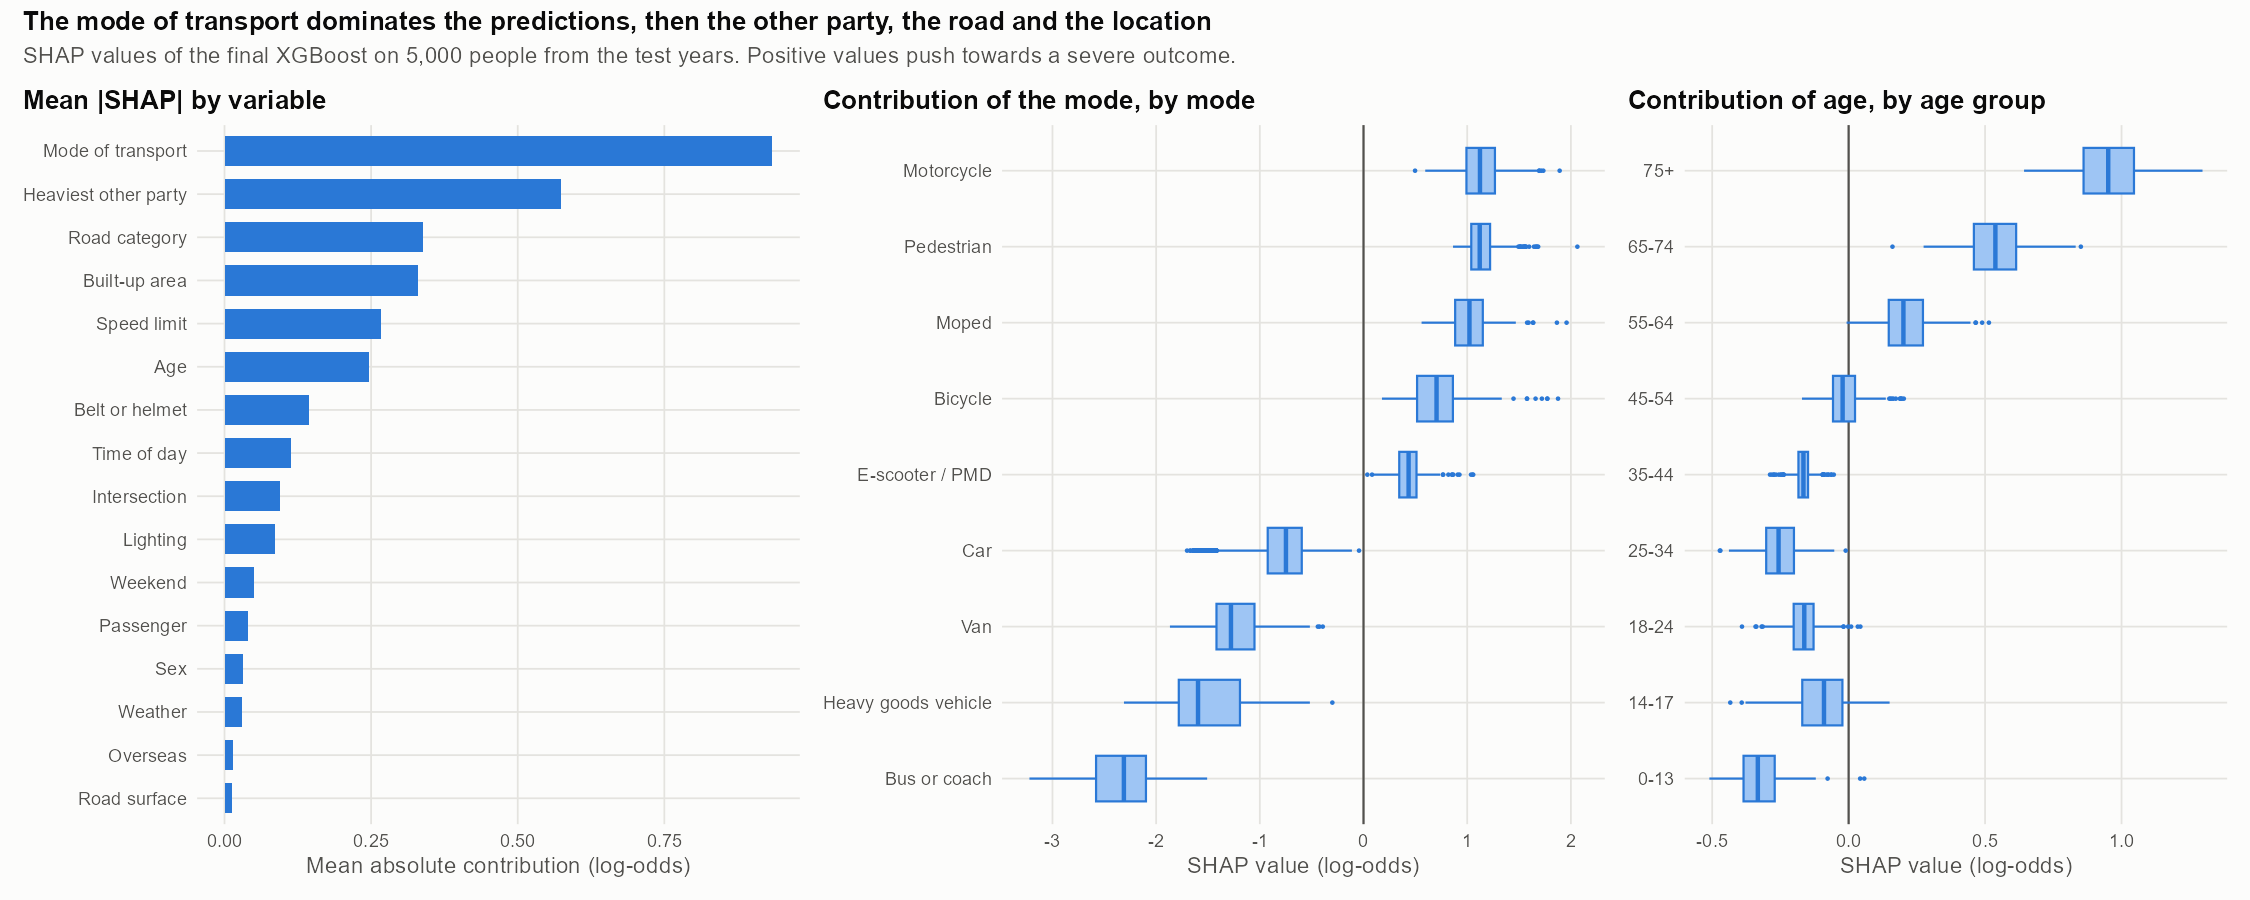
\includegraphics[width=\textwidth]{07_evaluation/05_shap.png}
\caption{SHAP values of the final XGBoost on 5,000 people from 2024--2025. Positive values push towards
a severe outcome.}
\label{fig:shap}
\end{figure}

%==========================================================================================
\section{Interactive dashboard}

A Quarto dashboard written in Observable JS presents the results without a server. Filters by years,
department and mode update the key figures, the yearly series, the severity by mode, the department
ranking and two maps (deaths per million inhabitants and per 100 accidents); a third page summarises the
odds ratios, the model scores and the SHAP importance. The data is pre-aggregated (1.2\,MB) so that the
page stays light, and the site is built into a folder ready for GitHub Pages.

%==========================================================================================
\section{Discussion and conclusion}

\paragraph{Main results.} The mode of transport decides most of the outcome: pedestrians, motorcyclists and
cyclists are several times more likely than car occupants to be killed or hospitalised in the same
situation. The other party and the place come next: heavy goods vehicles, roads outside built-up areas,
departmental roads, night-time and old age all raise the risk, and not wearing a belt or helmet multiplies
the odds by about four. Darkness and sex matter much less than raw rates suggest, and geography is about
road type more than population.

\paragraph{Statistics and machine learning.} Both approaches agree on what matters. The regression gives
interpretable effects with valid confidence intervals; XGBoost predicts slightly better because it
captures interactions without specifying them. For a public-health message the regression is the better
tool; for ranking cases, XGBoost.

\paragraph{Limits.} Only injury accidents are recorded, so nothing here measures the risk of having an
accident. Without exposure data, deaths per mode cannot be turned into a risk per kilometre. The
``hospitalised'' category changed in 2018, equipment use may be recorded more carefully when someone is
badly hurt, and hit-and-run users lack information. Speed, alcohol and drugs are not in the open data,
which limits prediction within a mode. Finally, odds ratios are adjusted associations, not causal effects.

\paragraph{Perspectives.} Adding exposure data (traffic counts, mobility surveys) to estimate risks per
kilometre, modelling the full ordinal severity scale, adding department random effects, using the
coordinates to locate dangerous road sections, and updating the pipeline each year with the new ONISR
release.

\paragraph{Reproducibility.} The project is a sequence of R scripts (download, harmonisation, quality,
features, exploration, geography, regression, machine learning, evaluation, dashboard data) run in order
by one command, followed by the Quarto render of the dashboard and the full report. Every number in this
report is produced by the code.

\begin{thebibliography}{9}
\small
\bibitem{onisr} ONISR. \emph{Bases de données annuelles des accidents corporels de la circulation
routière, années 2005 à 2025}. data.gouv.fr, Licence Ouverte 2.0.
\bibitem{cameron} A.\,C. Cameron and D.\,L. Miller. A practitioner's guide to cluster-robust inference.
\emph{Journal of Human Resources}, 50(2):317--372, 2015.
\bibitem{glmnet} J. Friedman, T. Hastie and R. Tibshirani. Regularization paths for generalized linear
models via coordinate descent. \emph{Journal of Statistical Software}, 33(1):1--22, 2010.
\bibitem{ranger} M.\,N. Wright and A. Ziegler. ranger: a fast implementation of random forests for high
dimensional data in C++ and R. \emph{Journal of Statistical Software}, 77(1):1--17, 2017.
\bibitem{xgboost} T. Chen and C. Guestrin. XGBoost: a scalable tree boosting system. \emph{Proceedings of
KDD}, 785--794, 2016.
\bibitem{shap} S.\,M. Lundberg and S.-I. Lee. A unified approach to interpreting model predictions.
\emph{Advances in Neural Information Processing Systems}, 30, 2017.
\end{thebibliography}

\end{document}
